\documentclass[11pt]{article}

% Increase main memory size
\usepackage{etex}
\usepackage{morewrites}
\usepackage{multicol}
\usepackage{pgfplots}
\usepackage{tikz}
\usetikzlibrary{external}
\tikzexternalize[prefix=cached_models/]

\usepackage{etex}
\usepackage{morewrites}
\usepackage{enumitem}
\usepackage{float}

\listfiles

\usepackage{amsmath, amssymb, amsthm}
\usepackage{graphicx}
\usepackage{geometry}
\usepackage{array}
\usepackage{booktabs}
\usepackage{float}
\usepackage{verbatim}
\usetikzlibrary{3d}

% Page Layout
\geometry{a4paper, margin=1in}
\setlength\parindent{0pt}
\pgfplotsset{compat=1.18}

% Custom commands
\newcommand{\card}[1]{\lvert #1 \rvert}
\newcommand{\inner}[2]{\left\langle #1, #2 \right\rangle}

\title{\textbf{Exercises in Principles of Mathematical Analysis}}
\author{}
\date{}

\begin{document}

\maketitle

\section*{Exercise 1.1.1}
\textbf{\large Prove that \(\mathbb{Q}\) has zero measure.}

A set \(Q \subset \mathbb{R}\) has measure zero if and only if:
\[Q \subset \bigcup_{j=1}^{\infty} A_j, \quad \text{where } A_j \text{ are intervals and } \sum_{j=1}^{\infty} \card{A_j} < \varepsilon, \forall \epsilon > 0.\]

Since \(\mathbb{Q}\) is countable, we can enumerate its elements as \(\{q_1, q_2, q_3, \ldots\}\). 

We start with:
\[\sum_{j=1}^{\infty} \dfrac{1}{2^{j}} = \dfrac{1/2}{1 - 1/2} = 1.\]

Then, we can multiply this series by any \(\epsilon > 0\) to get:
\[\sum_{j=1}^{\infty} \dfrac{\epsilon}{2^{j}} = \varepsilon.\]

For each rational number \(q_j\), we can construct an interval \(A_j\) centered at \(q_j\) with length \(\dfrac{\varepsilon}{2^{j}}\):
\[A_j = \left(q_j - \dfrac{\varepsilon}{2^{j+1}}, q_j + \dfrac{\varepsilon}{2^{j+1}}\right).\]

Thus, we have:
\[\mathbb{Q} \subset \bigcup_{j=1}^{\infty} A_j, \quad \text{and } \sum_{j=1}^{\infty} \card{A_j} = \sum_{j=1}^{\infty} \dfrac{\varepsilon}{2^{j}} = \varepsilon.\]

Since \(\varepsilon\) can be made arbitrarily small, we conclude that \(\mathbb{Q}\) has measure zero.

\begin{center}
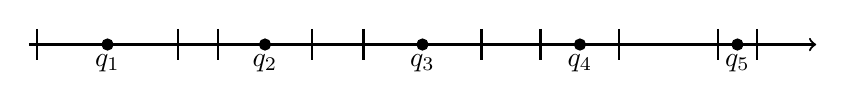
\begin{tikzpicture}
    % Draw the real line
    \draw[thick, ->] (-5, 0) -- (5, 0) node[right] {};
    
    % Place rational points q_i
    \foreach \x/\label in {-4/{$q_1$}, -2/{$q_2$}, 0/{$q_3$}, 2/{$q_4$}, 4/{$q_5$}} {
        \filldraw (\x, 0) circle (2pt) node[below] {\label};
    }
    
    % Draw intervals around q_i as parentheses
    \foreach \x/\len in {-4/0.9, -2/.6, 0/0.75, 2/0.5, 4/0.25} {
        \draw[thick] (\x-\len, 0.2) -- (\x-\len, -0.2);
        \draw[thick] (\x+\len, 0.2) -- (\x+\len, -0.2);
    }
\end{tikzpicture}
\end{center}

\pagebreak
\section*{Exercise 1.1.2}
\textbf{\large For the following function defined on \([0,1]\):
\[f(x) = \begin{cases} 
\dfrac{1}{q} & \text{if } x = \dfrac{p}{q}, \quad p, q \in \mathbb{Z}, q \neq 0 \\
0 & \text{if } x \notin \mathbb{Q}
\end{cases}\]
\begin{enumerate}
    \item Show that \(f\) is discontinuous only at the rational points.
    \item Prove that \(f\) is Riemann integrable.
\end{enumerate}}
\vskip 1em
\begin{center}
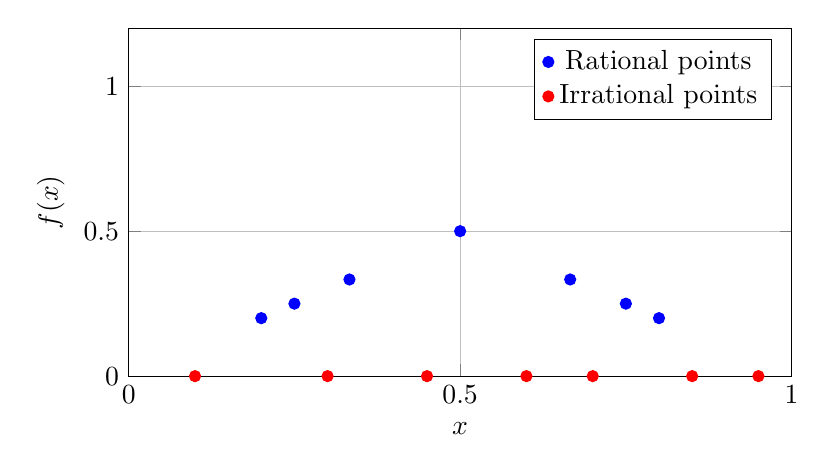
\begin{tikzpicture}
    \begin{axis}[
        width=10cm,
        height=6cm,
        xlabel={$x$},
        ylabel={$f(x)$},
        ymin=0, ymax=1.2,
        xmin=0, xmax=1,
        domain=0:1,
        samples=100,
        ytick={0, 0.5, 1},
        xtick={0, 0.5, 1},
        grid=both,
        legend pos=north east
    ]
        % Plot random points for rationals
        \addplot[only marks, mark=*, color=blue] coordinates {
            (0.2, 1/5) (0.25, 1/4) (0.333, 1/3) (0.5, 1/2) (0.666, 1/3) (0.75, 1/4) (0.8, 1/5)
        };
        \addlegendentry{Rational points}

        % Plot random points for irrationals
        \addplot[only marks, mark=*, color=red] coordinates {
            (0.1, 0) (0.3, 0) (0.45, 0) (0.6, 0) (0.7, 0) (0.85, 0) (0.95, 0)
        };
        \addlegendentry{Irrational points}
    \end{axis}
\end{tikzpicture}
\end{center}

If $x$ is irrational, then
\[\lim_{x \to x_0} f(x) \stackrel{?}{=} 0 = f(x_0),\]

$\forall \varepsilon > 0$, we want $\card{f(x) - 0} = \card{f(x)} < \varepsilon$ if $x$ is close enough to $x_0$ i.e. $x \in \left(x_0 - \delta, x_0 + \delta\right)$ for some $\delta > 0$.

For example, take $\varepsilon = \dfrac{1}{3}$, then $\card{f(x)} < \dfrac{1}{3}$ if $f(x) = \dfrac{1}{q} < \dfrac{1}{3} \Rightarrow q > 3$. So, except for the rationals $0, 1, \dfrac{1}{2}, \dfrac{1}{3}, \dfrac{2}{3}$, we have $\card{f(x)} < \varepsilon = \dfrac{1}{3}$. 
We can do this for any $\varepsilon > 0$ by choosing $q > \dfrac{1}{\varepsilon}$, so 
\[\lim_{x \to x_0} f(x) = 0.\]

So it is continuous at every irrational point. On $\mathbb{Q}$, the value of $f(x)$ is non-zero, so it is discontinuous at every rational point.

Finally, since the set of discontinuities has measure zero ($\card{\mathbb{Q}} = 0$), $f$ is Riemann integrable.

\pagebreak
\section*{Exercise 1.1.4}
\textbf{\large Consider the sequence of functions given by:
\[f_n(x) = \begin{cases}
1 & \text{if } \card{x} \leq n \\
0 & \text{if } \card{x} > n
\end{cases}\]
Obtain the limit \(\lim_{n \to \infty} f_n(x)\) and study whether the convergence is uniform or not.}
\[\sup_{n \in \mathbb{N}} \card{f_n(x) - f(x)} = 1 \neq 0, \quad \forall x \in \mathbb{R}.\]
So the convergence is not uniform.

\section*{Exercise 1.1.5}
\textbf{\large Prove that the following series converges in \([0,1]\). Is the convergence uniform?}
\[\sum_{n=0}^{\infty} x(1 - x)^n = x \sum_{n=0}^{\infty} (1 - x)^n = \begin{cases}
\dfrac{x}{1 - (1 - x)} = \dfrac{x}{x} = 1 & \text{if } x \in (0, 1) \\
0 & \text{if } x = 0 \\
0 & \text{if } x = 1
\end{cases}
\]

If \(\card{1 - x} < 1\), then the series converges. This is true for all \(x \in [0,1]\). The convergence is not uniform since $f$ is not continuous:
\[f_N(x) = \sum_{n=0}^{N} x(1 - x)^n \stackrel{N \to \infty}{\longrightarrow} f(x) = \begin{cases}
1 & \text{if } x \in (0, 1) \\
0 & \text{if } x = 0 \\
0 & \text{if } x = 1
\end{cases}
\]

\section*{Exercise 1.1.3}
\textbf{\large Prove that if a function \(f: [a,b] \to \mathbb{R}\) is monotonus, then it:
\begin{enumerate}
    \item is bounded
    \item is Riemann integrable.
\end{enumerate}}

Suppose \(f\) is monotonically increasing. Then,
\[f(x) \in [f(a), f(b)], \quad \forall x \in [a,b].\]
So \(f\) is bounded.

Now, we build $U_f(P)$ and $L_f(P)$ for a partition $P = \{a, a + \dfrac{b-a}{n}, a + 2\dfrac{b-a}{n}, \ldots, b\}$.
\[U_f(P) = \sum_{i=1}^{n} \sup_{x \in [x_{i-1}, x_i]} f(x) \cdot (x_i - x_{i-1}) = \sum_{i=1}^{n} f(x_i) \cdot \dfrac{b-a}{n},\]
\[L_f(P) = \sum_{i=1}^{n} \inf_{x \in [x_{i-1}, x_i]} f(x) \cdot (x_i - x_{i-1}) = \sum_{i=1}^{n} f(x_{i-1}) \cdot \dfrac{b-a}{n}.\]
Then,
\[U_f(P) - L_f(P) = \dfrac{b-a}{n} \sum_{i=1}^{n} \left(f(x_i) - f(x_{i-1})\right) = \dfrac{b-a}{n} \left(f(b) - f(a)\right) \stackrel{n \to \infty}{\longrightarrow} 0.\]
So \(f\) is Riemann integrable. 

\end{document}
